\documentclass[10.7pt,a4paper]{letter}
\usepackage[top=.75in, bottom=.75in, left=.75in, right=0.75in]{geometry}
\usepackage{graphicx}
\usepackage{natbib}
\address{1300 Centre Street \\ Boston, MA, 20131}
\begin{document}
\bibliographystyle{..//..//refs/bibstyles/amnat.bst}
\begin{letter}{}
\includegraphics[width=0.3\textwidth]{/Users/aileneettinger/Dropbox/Documents/Work/AA_heading.pdf}
\pagenumbering{gobble}

\opening{Dear Dr. Findlay:}
We propose a ``Perspective" on implications of the altered photoperiod that many organisms will experience as they shift their ranges or seasonal activities with climate change. We believe this piece would be of broad interest to readers of \emph{Nature Climate Change} because shifts in photoperiod would have wide-reaching impacts on many plant and animal species. Photoperiod acts as a cue for the spring emergence and migration timing of diverse species, and alterations to experienced photoperiod can affect development, growth, and fitness for plants, insects, fish, and mammals, among other organisms. Thus, understanding these changes is critical for biologists forecasting species responses, policy-makers dependent on these forecasts for adaptation strategies, and those dependent on the services provided by these species. Yet, photoperiod has rarely been included in forecasts of responses to climate change and implications of climate-change-induced shifts in photoperiod are largely unexplored, especially for early-season spring events, where changes will be most dramatic. 
\\
\\
The two most-observed impacts of climate change on species are shifts in space (altitudinal and latitudinal range shifts) and in time (phenological shifts) (\emph{1,2}); both result in altered photoperiod regimes (\emph{3}).  Altered photoperiods have the potential to dramatically alter species' performance and fitness, however, the magnitude of effects of shifts in photoperiod with climate change are unknown or unquantified for the vast majority of species.  Our ``Perspective" would quantify expected changes in experienced photoperiod due to shifts in space versus in time, given observations to date (e.g., \emph{1,2}), and put them in a novel, global context. Previous work has focused on effects geographic shifts in species distributions on photoperiod (e.g., \emph{3,4}), yet we will demonstrate that impacts on experienced photoperiod due to temporal shifts may be orders of magnitude larger than impacts due to spatial shifts (e.g., 1.6 hours of change versus one minute of change, Fig. 1). 
\\
\\
Our ``Perspective" would also offer a valuable addition to current approaches because it would focus on spring phenology events. To date, the role of photoperiod has received far more detailed attention for end-of-season activities, such as growth cessation in the fall, than for spring activities. Though photoperiod cues dominate in the fall for many organisms, fall phenology responses to climate change have been muted. In contrast, spring phenology responds strongly to temperature and thus has advanced substantially with warming---causing cascading, and generally unexplored, effects on photoperiod experienced at the start of spring. With continued warming photoperiod limitations could come into play, however, and cause the rapidly advancing springs to abruptly slow or stall. We will demonstrate that incorporating photoperiod into forecasts is possible by leveraging existing experimental data: for example, growth chamber experiments on woody plant spring phenology often have data relevant for climate change impacts (e.g., Fig. 2). We plan to highlight how new modeling approaches can improve predictions of when, where, and how much photoperiod is likely to affect future spring phenology and could be combined with new empirical work to advance our understanding of the role of photoperiod in a warming world. 
\\
\\
We expect the title of our manuscript to be ``Spatial and temporal shifts in photoperiod with climate change."  It will be co-authored by D. Buonaiuto, C. Chamberlain, I. Morales-Castilla, and E. Wolkovich. Thank you for considering our paper.

Sincerely,\\
\includegraphics[scale=.4]{/Users/aileneettinger/Dropbox/Documents/Work/AileneEttingerSignature.png} \\
Ailene Ettinger
\\
\begin{footnotesize}
NRC Research Associate, Northwest Fisheries Science Center
\\
Visiting Fellow, Arnold Arboretum of Harvard University
\end{footnotesize}
\\
\newpage
\noindent \emph{References in letter}
\begin{footnotesize}
\begin{enumerate}
\item Chen, I.-C., J. K. Hill, R. Ohlemueller, D. B. Roy, and C. D. Thomas. 2011. Rapid range shifts of species associated with high levels of climate warming.  \emph{Science} 333:1024-1026.
\item Parmesan, C. and Yohe, G., 2003. A globally coherent fingerprint of climate change impacts across natural systems.  \emph{Nature}, 421:37.

\item Saikkonen, K., K. Taulavuori, T. Hyvonen, P. E. Gundel, et al. 2012. Climate change-driven species' range shifts filtered by photoperiodism. \emph{Nature Climate Change} 2:239.
\item Way, D. A., and R. A. Montgomery. 2015. Photoperiod constraints on tree phenology, performance and migration in a warming world. \emph{Plant, Cell \& Environment} 38:1725-1736.
\item Parmesan, C., 2006. Ecological and evolutionary responses to recent climate change.  \emph{Annu. Rev. Ecol. Evol. Syst.}, 37: 637-669.
\item Wolkovich, E., A. Ettinger, D. Flynn, T. Savas, C. Chamberlain, et al. 2019. Observed Spring Phenology Responses in Experimental Environments (OSPREE). Knowledge Network for Biocomplexity. urn:uuid:b2ab2746-b830-436b-a7a9-01b3ef3558e4. (Currently only metadata is available.)
\end{enumerate}

\begin{figure}
\centering
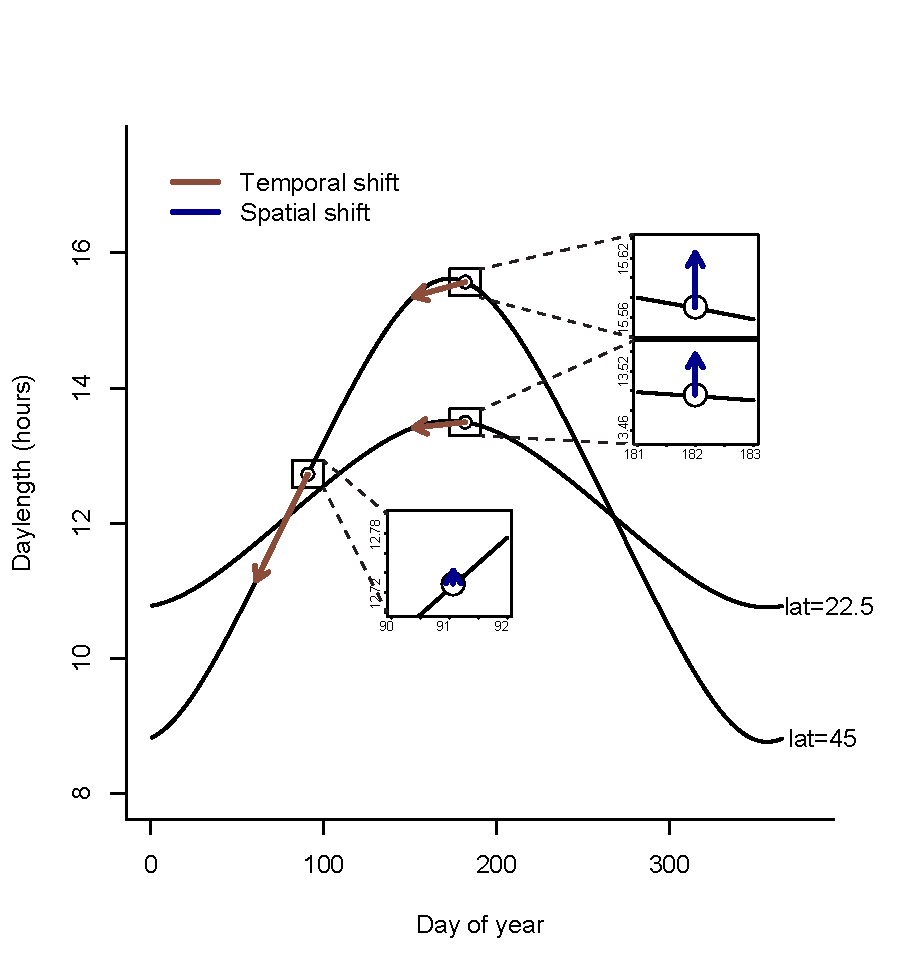
\includegraphics[width=90mm,scale=0.5]{..//..//analyses/photoperiod/figures/photo_spacetime_v2.pdf} \\

\caption{Figure 1: Photoperiod varies with latitude and by day of year, such that temporal shifts in activity yield larger changes in experienced photoperiod compared with spatial shifts. Here, we show this variation at two latitudes (22.5\degree, 45\degree), using hypothetical spatial and temporal shifts. These shifts,
which are similar to observed average rates with recent global warming (e.g., \emph{1,5}), highlight the greater magnitude in daylength changes close to the equinox (e.g., day of
year 91), versus close to the summer solstice (e.g., day of year 182).}
 \label{fig:condiag}
 \end{figure}
 
 \begin{figure}
\centering
\includegraphics[width=130mm,scale=0.5]{..//..//analyses/photoperiod/figures/ospree_photopmap_fromblake.jpg} 

\caption{Figure 2. Experimental photoperiod treatments and their equivalent spatial and temporal shifts for growth chamber experiments that manipulate photoperiod, compiled in a new database (\emph{6}). To calculate the required spatial (lines) or temporal (symbols) shifts for each experiment, we used observed rates with recent warming: 16.9 kilometers per decade (or approximately 1.5 degrees in 100 years) for spatial shifts (\emph{1}) and 2.3 days per decade (or 23 days in 100 years) for temporal shifts (\emph{2}).}
 \label{fig:photomap}
 \end{figure}


\end{footnotesize}
\end{letter}
\end{document}
